\documentclass[final]{beamer}\usepackage[]{graphicx}\usepackage[]{color}
%% maxwidth is the original width if it is less than linewidth
%% otherwise use linewidth (to make sure the graphics do not exceed the margin)
\makeatletter
\def\maxwidth{ %
	\ifdim\Gin@nat@width>\linewidth
	\linewidth
	\else
	\Gin@nat@width
	\fi
}
\makeatother

\definecolor{fgcolor}{rgb}{0.345, 0.345, 0.345}
\newcommand{\hlnum}[1]{\textcolor[rgb]{0.686,0.059,0.569}{#1}}%
\newcommand{\hlstr}[1]{\textcolor[rgb]{0.192,0.494,0.8}{#1}}%
\newcommand{\hlcom}[1]{\textcolor[rgb]{0.678,0.584,0.686}{\textit{#1}}}%
\newcommand{\hlopt}[1]{\textcolor[rgb]{0,0,0}{#1}}%
\newcommand{\hlstd}[1]{\textcolor[rgb]{0.345,0.345,0.345}{#1}}%
\newcommand{\hlkwa}[1]{\textcolor[rgb]{0.161,0.373,0.58}{\textbf{#1}}}%
\newcommand{\hlkwb}[1]{\textcolor[rgb]{0.69,0.353,0.396}{#1}}%
\newcommand{\hlkwc}[1]{\textcolor[rgb]{0.333,0.667,0.333}{#1}}%
\newcommand{\hlkwd}[1]{\textcolor[rgb]{0.737,0.353,0.396}{\textbf{#1}}}%
\let\hlipl\hlkwb

\usepackage{framed}
\makeatletter
\newenvironment{kframe}{%
	\def\at@end@of@kframe{}%
	\ifinner\ifhmode%
	\def\at@end@of@kframe{\end{minipage}}%
\begin{minipage}{\columnwidth}%
	\fi\fi%
	\def\FrameCommand##1{\hskip\@totalleftmargin \hskip-\fboxsep
		\colorbox{shadecolor}{##1}\hskip-\fboxsep
		% There is no \\@totalrightmargin, so:
		\hskip-\linewidth \hskip-\@totalleftmargin \hskip\columnwidth}%
	\MakeFramed {\advance\hsize-\width
		\@totalleftmargin\z@ \linewidth\hsize
		\@setminipage}}%
{\par\unskip\endMakeFramed%
	\at@end@of@kframe}
\makeatother

\definecolor{shadecolor}{rgb}{.97, .97, .97}
\definecolor{messagecolor}{rgb}{0, 0, 0}
\definecolor{warningcolor}{rgb}{1, 0, 1}
\definecolor{errorcolor}{rgb}{1, 0, 0}
\newenvironment{knitrout}{}{} % an empty environment to be redefined in TeX

\usepackage{alltt}
\usepackage[scale=1.20]{beamerposter} % Use the beamerposter package for laying out the poster
\usetheme{confposter} % Use the confposter theme supplied with this template
\setbeamercolor{block title}{fg=DarkOrchid,bg=white} % Colors of the block titles
\setbeamercolor{block body}{fg=black,bg=white} % Colors of the body of blocks
\setbeamercolor{block alerted title}{fg=white,bg=BrewerBlue1} % Colors of the highlighted block titles
\setbeamercolor{block alerted body}{fg=black,bg=dblue!10} % Colors of the body of highlighted blocks
% Many more colors are available for use in beamerthemeconfposter.sty

%-----------------------------------------------------------
% Define the column widths and overall poster size
% To set effective sepwid, onecolwid and twocolwid values, first choose how many columns you want and how much separation you want between columns
% In this template, the separation width chosen is 0.024 of the paper width and a 4-column layout
% onecolwid should therefore be (1-(# of columns+1)*sepwid)/# of columns e.g. (1-(4+1)*0.024)/4 = 0.22
% Set twocolwid to be (2*onecolwid)+sepwid = 0.464
% Set threecolwid to be (3*onecolwid)+2*sepwid = 0.708

\newlength{\sepwid}
\newlength{\onecolwid}
\newlength{\twocolwid}
\newlength{\threecolwid}
\setlength{\paperwidth}{45in} % A0 width: 46.8in
\setlength{\paperheight}{36in} % A0 height: 33.1in
\setlength{\sepwid}{0.01\paperwidth} % Separation width (white space) between columns
\setlength{\onecolwid}{0.24\paperwidth} % Width of one column
\setlength{\twocolwid}{0.464\paperwidth} % Width of two columns
\setlength{\threecolwid}{0.708\paperwidth} % Width of three columns
\setlength{\topmargin}{-0.5in} % Reduce the top margin size
%-----------------------------------------------------------

\usepackage{graphicx}  % Required for including images
\usepackage{booktabs} % Top and bottom rules for tables

\setbeamerfont{caption}{size=\scriptsize} 

\renewcommand\figurename{Fig.}

\usepackage{FiraSans}

\title{ You keep using Coefficient of Variation\\ \emph{I do not think it means what you think it means }  }
%\subtitle{Inigo Montoya suggests variance partitioning, instead}

\author{Devan Allen McGranahan \inst{1} \and Samuel D. Fuhlendorf \inst{2}}
\institute{\inst{1} USDA Agricultural Research Service, Miles City, MT; 
                      \inst{2} Oklahoma State University, Stillwater, OK}
\IfFileExists{upquote.sty}{\usepackage{upquote}}{}
\begin{document}
%\SweaveOpts{concordance=TRUE}


\addtobeamertemplate{block end}{}{\vspace*{2ex}} % White space under blocks
\addtobeamertemplate{block alerted end}{}{\vspace*{2ex}} % White space under highlighted (alert) blocks

\setlength{\belowcaptionskip}{2ex} % White space under figures
\setlength\belowdisplayshortskip{2ex} % White space under equations

\begin{frame}[t] % The whole poster is enclosed in one beamer frame

\begin{columns}[t] % The whole poster consists of three major columns, the second of which is split into two columns twice - the [t] option aligns each column's content to the top

\begin{column}{\sepwid}\end{column} % Empty spacer column

\begin{column}{\onecolwid} % The first column


%	OBJECTIVES
\vspace{-1cm}
\begin{alertblock}{	Overview }
	
\begin{itemize}
	\item Variability\textemdash statistically, \emph{variance}, the second data moment\textemdash can be a more important ecological property than the mean 
\item Coefficient of Variation is popular but problematic under multiple sources of variability 
\item \textbf{We demonstrate \emph{variance partitioning} as a spatially-explicit alternative to CV}
\end{itemize} 
\end{alertblock}

\begin{block}{Defining variability}
\begin{itemize}
	\item[] \textbf{Coefficient of Variation}
\item Variability can be abstract\textemdash simple measures are understandable 
\item Coefficient of Variation is calculated as \\
%\begin{equation*}
	$CV = \frac{\sigma}{\mu} \cdot 100 $ 
%\end{equation*}
\item[] where $\sigma$ = standard deviation and $\mu$ = mean
\item[] \textbf{Handling multiple sources of variability} 
\item \emph{CV is only reliable when mean is constant}
\item When variability effects differences in both $\mu$ and $\sigma$, CV is misleading
\item Both \emph{inherent} and \emph{disturbance-driven heterogeneity} can case variability in $\mu$ and $\sigma$:
\end{itemize}

\begin{figure}
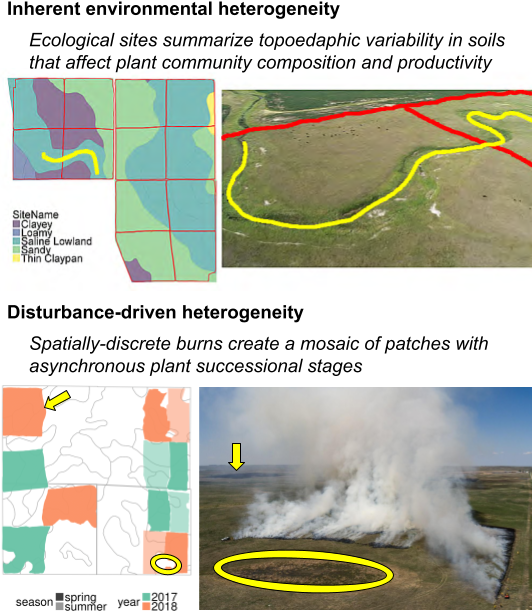
\includegraphics[width=8.5in]{figure/HeterogeneitySources}
\caption{~Examples of heterogeneity sources.}
\label{HetSources}
\end{figure}

\end{block}
\end{column} 
% End of the first column

%------------------------------------------------

\begin{column}{\sepwid}\end{column} % Left spacer column

\begin{column}{\twocolwid} % Begin a column two columns wide (column 2)

\begin{columns}[T] % align columns
	
\begin{column}{0.4\textwidth} % Begin left half of central column

	\vspace{-2.5cm}	
	\begin{alertblock}{Data and methods}
		\small{
		\raggedright
		\emph{Productivity Scenarios} defined by quantiles of the range of productivity across US National Grasslands as determined by Rangeland Analysis Platform data on perennial + annual herbaceous biomass
		\begin{center}
			\begin{figure}
	
			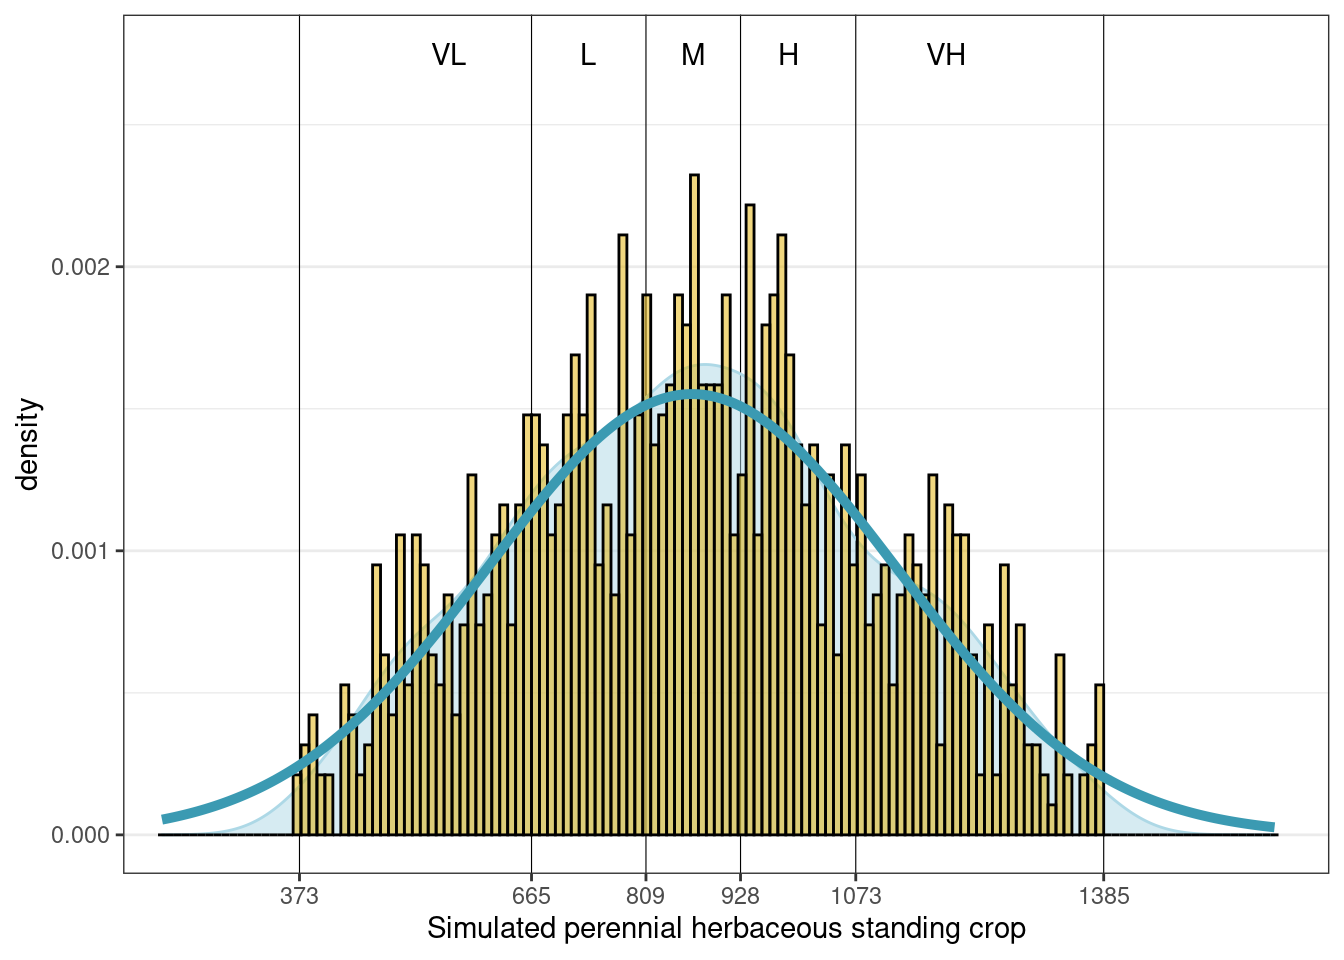
\includegraphics[]{figure/NonSpatialData}
			\caption{~Productivity classes (kg ha\textsuperscript{-1}).}
			\label{productivity}
		\end{figure}
		\begin{tabular}{l ccc}
			\toprule
			\textbf{Productivity scenario} & \textbf{Mean} & \textbf{SD} & \textbf{CV}  \\ \midrule
			Very Low (VL)	&	553 & 78.8 & 	0.14 \\
			Low (L) &	739 &	42.3 &	0.06 \\
			Medium (M) &	869 & 33.6 &	0.04 \\
			High (H) &	993 &	39.4 &	0.04\\
			Very High (VH) & 1194 & 81.7 & 0.07 \\ \bottomrule
		\end{tabular}
	\end{center}
	\textbf{Non-spatial simulations}
	
	Calculate CV for each productivity scenario:
	\begin{itemize}
		\item Actual mean ($\mu$) and standard deviation ($\sigma$) from data in Fig.~\ref{productivity}. 
		\item Constant $\mu$ across productivity classes (VH \& VL) with $\sigma$ from each class
		\item Constant $\sigma$ across productivity classes (VH \& VL) with $\mu$ from each class
	\end{itemize}
\textbf{Spatial simulations}

Four landscape scenarios (Fig.~\ref{SpatialData}):
\begin{itemize}
	\item Randomly-distributed productivity
	\item Disturbance only: Time-since-fire gradient
	\item Inherent variability only: soil types
	\item Both disturbance gradient and soil types
\end{itemize}
		\begin{center}
	\begin{figure}
		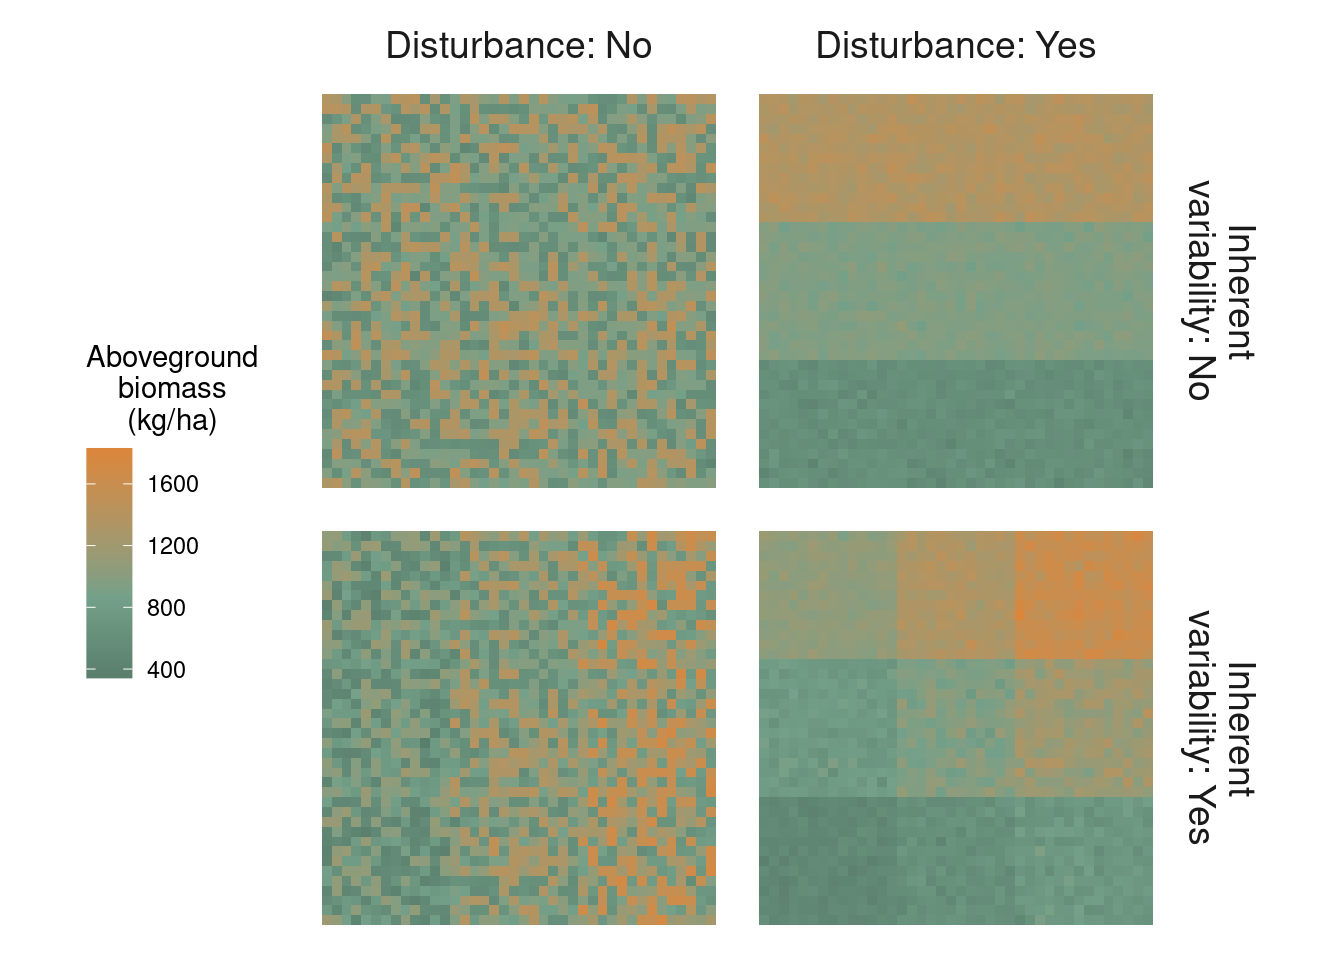
\includegraphics[]{figure/SpatialData}
		\caption{~Four simulated landscapes.}
		\label{SpatialData}
	\end{figure}
\end{center}		}
		
	\end{alertblock} 


\end{column}% End left half of central column
\hfill%
\begin{column}{0.6\textwidth} % Begin right half of central column
	\vspace{-2cm}
		\begin{block}{Problems with CV} \end{block}
\vspace{-1cm}
\textbf{Non-spatial example}
\begin{itemize}
	\item When means vary, \emph{CV declines as mean increases}
	\item Low mean, high CV relationship \emph{independent of SD}
\end{itemize} 

\begin{figure}
	\begin{center}
		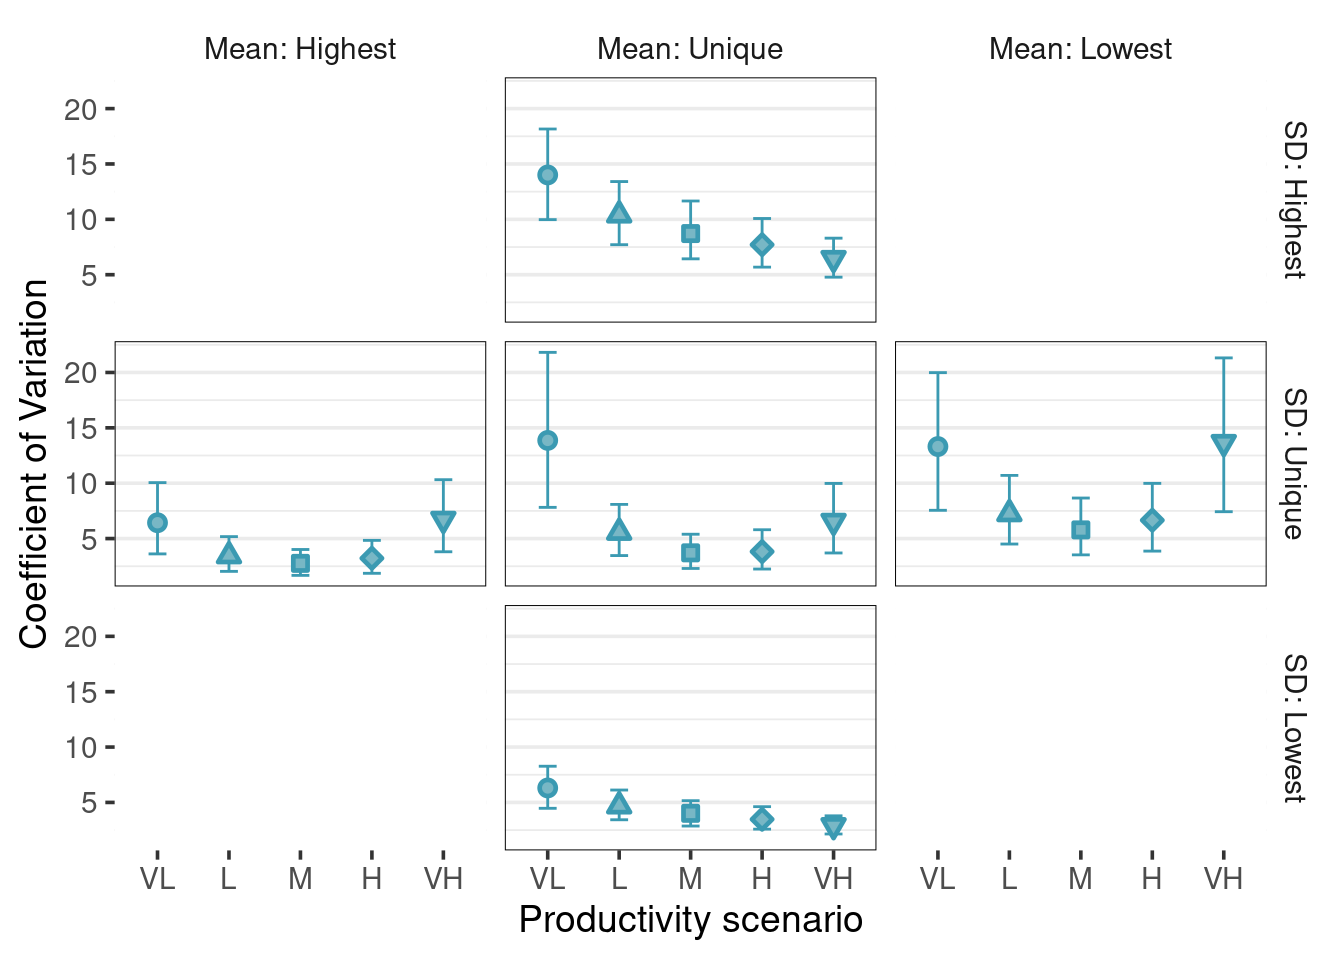
\includegraphics[width=1.5\maxwidth]{figure/NonSpatialResults}
		\caption{~CV calculations from non-spatial example. 
			\emph{Center:} CV with actual mean and SD for each productivity scenario (Fig.~\ref{productivity}). 
			\emph{L \& R:} CV with unique SD for each scenario and constant mean, highest and lowest classes. 
			\emph{Top \& Bottom:} CV with unique mean for each scenario and constant SD, highest and lowest classes.}
		\label{NonSpatialExample}
	\end{center}
\end{figure}

\textbf{Spatial example} 

\begin{itemize}
	\item CV is not sensitive to landscape-level heterogeneity
	\item Similar trends as in Fig.~\ref{SpatialData} when homoscedastic
\end{itemize} 

\begin{figure}
	\begin{center}
		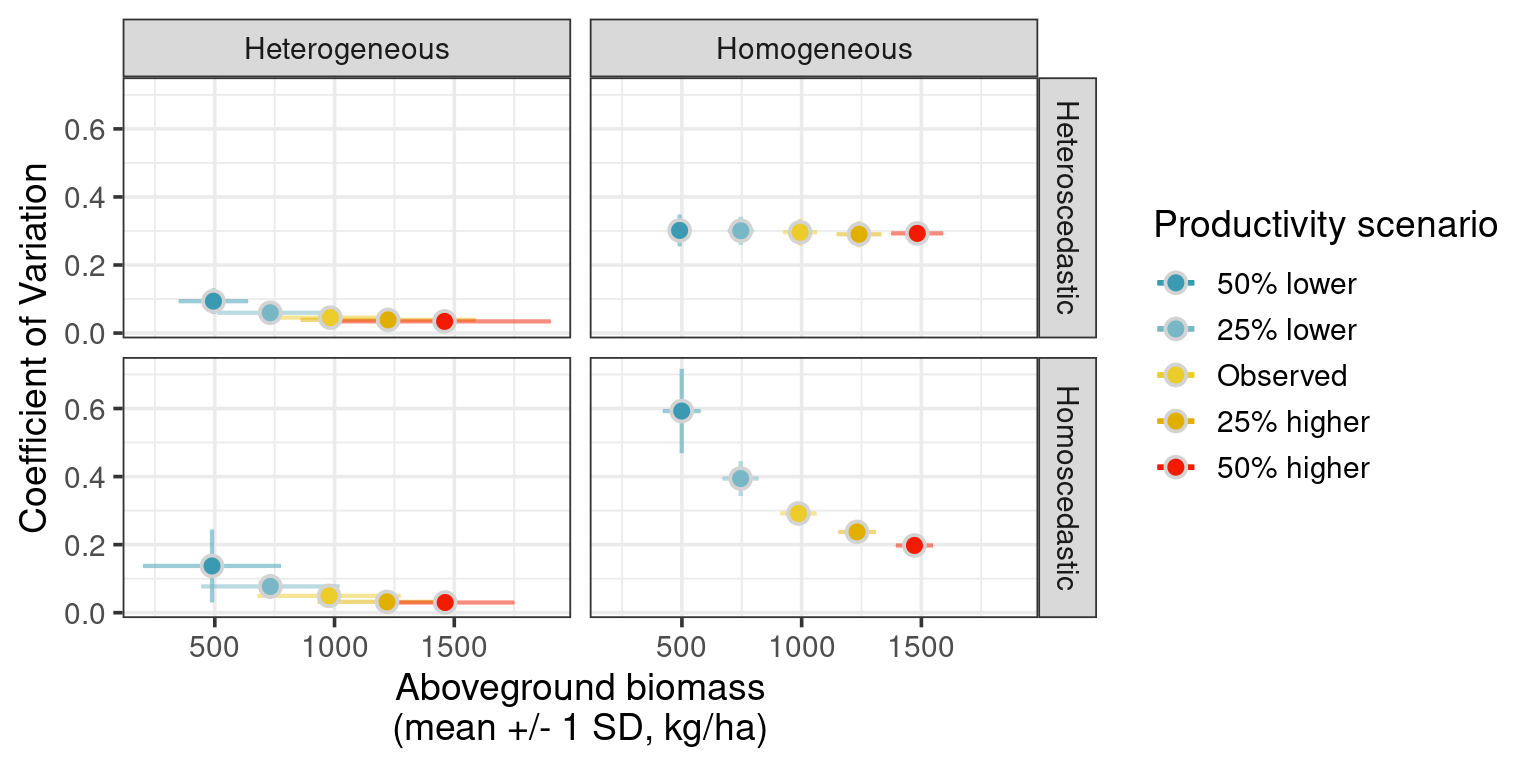
\includegraphics[width=1.5\maxwidth]{figure/SpatialResults}
		\caption{~\emph{Columns:} CV across heterogeneous and homogeneous landscapes (Fig.~\ref{SpatialData}). \emph{Rows:} Assuming the variance in productivity data remain constant as means increase (homoscedastic, and assumption of linear regression ) vs increasing variance with mean (heteroscedastic, a reality of many ecological data.)}
		\label{SpatialExample}
	\end{center}
\end{figure}

\end{column}%
\end{columns}  % End of the split of column 2

\end{column} % End of the central, split column

\begin{column}{\sepwid}\end{column} % Empty spacer column

\begin{column}{\onecolwid} % The third column
	\vspace{-1cm}
\begin{block}{Solution: Variance Partitioning} \end{block}
	\vspace{-2cm}
\begin{itemize}
	\item Random-effect regression parses variance into spatially-relevant scales
	\item Spatial heterogeneity \emph{quantified as patch contrast}\textemdash the degree of difference among landscape units
	\item Coarse distinction between heterogeneous (patchy) and homogeneous (uniform) landscapes
	\item Fine distinction among degrees of variability among patches
\end{itemize} 

\begin{figure}
	\begin{center}
		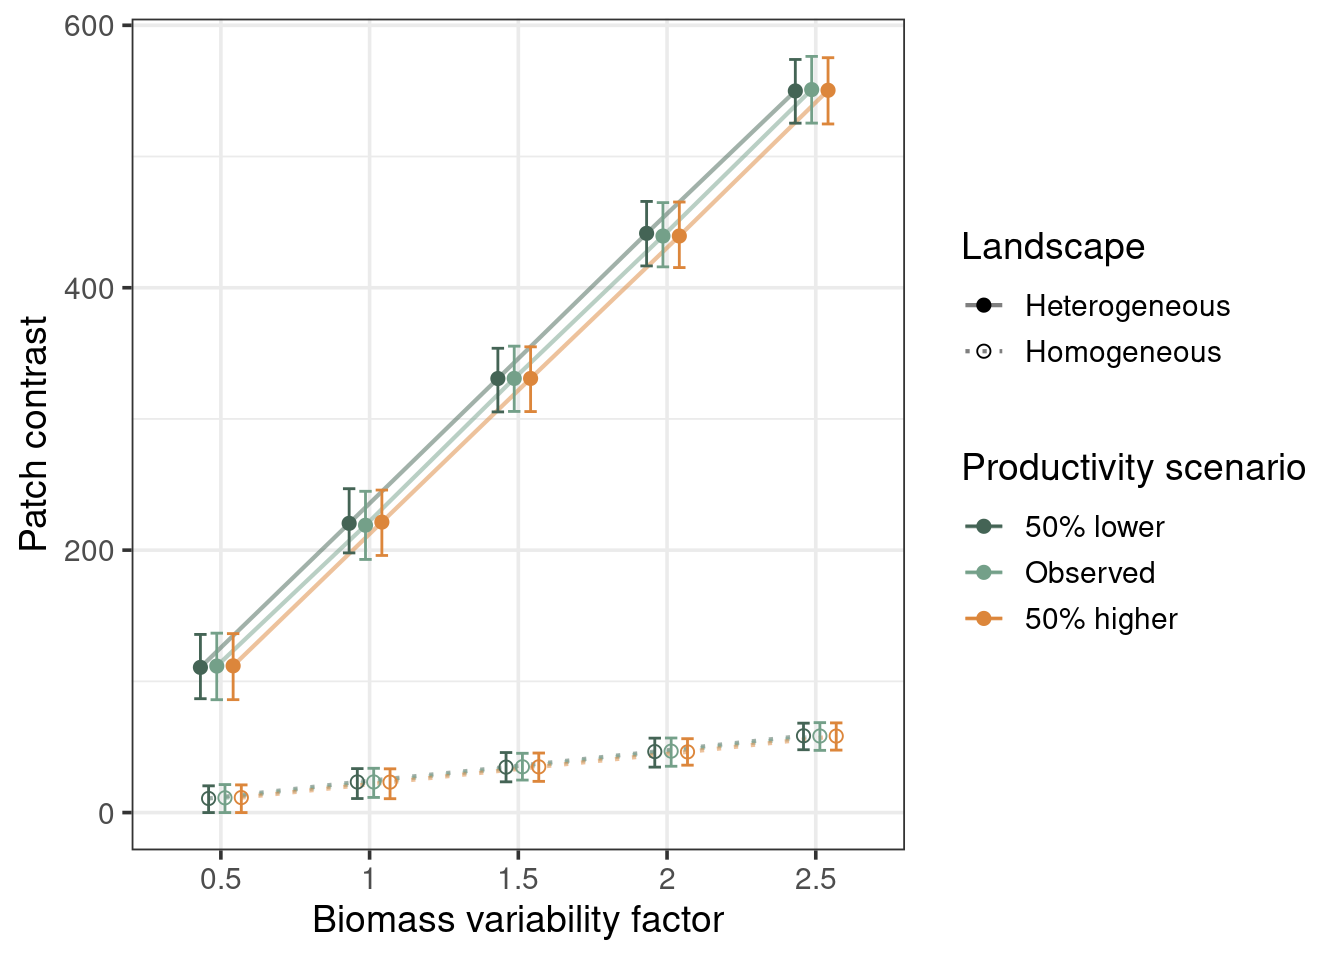
\includegraphics[width=1.5\maxwidth]{figure/VariancePartitioning}
		\caption{~The proportion variance attributable to the patch term in a random-effect regression\textemdash\emph{Patch Contrast}\textemdash within heterogeneous and homogeneous landscapes from Fig.~\ref{SpatialData}. }
		\label{VariancePartitioning}
	\end{center}
\end{figure}
	
\begin{alertblock}{\textbf{Avoid CV when means vary!}}

\begin{itemize}
\item CV is only useful to compare variability when mean values are constant. 
\item CV is not sensitive to spatial heterogeneity.
\item {Variance partitioning} is robust for data with spatial structure\textemdash always a good idea when sampling heterogeneous environments. 
\item Variance partitioning can be accomplished with \texttt{proc GLIMMIX} in SAS, \texttt{lme4::(g)lmer} in \textbf{R}. The \textbf{R} package \texttt{rptR} also performs variance decomposition.
\end{itemize}

\end{alertblock}

\end{column} % End of the third column

\end{columns} % End of all the columns in the poster

\end{frame} % End of the enclosing frame

\end{document}
